\chapter{Web aplikacija}

Svi podaci koji su pohranjeni u bazi podataka trebaju biti korisnicima na raspolaganju jednostavno i intuitivno. U tu je svrhu kreirana aplikacija radi prikaza i vizualizacije podataka korisnicima u stvarnom vremenu. Web aplikacija treba biti javno dostupna na internetu kako bi korisnici razvijenog sustava mogli pregledavati podatke poslane s uređaja. Za objavu web aplikacije na internet \engl{deployment} kreirani su vlastiti resursi na kojima se izvršava aplikacija. Za infrastrukturu aplikacije korišteni su resursi platforme AWS koji pružaju iznajmljivanje virtualnih računala te se na njima mogu pokrenuti vlastite računalne aplikacije. Za web aplikaciju koja će korisnicima pružati uvid u podatke odabrana je Grafana koja nudi brojne funkcionalnosti za vizualizaciju podataka. Nadalje, kreiran je i alarmni sustav koji obavještava o promjenama stanje koja dolaze od uređaja. 

\section{Infrastruktura aplikacije}

Temelj cijele infrastrukture aplikacije jest usluga Amazon EC2 \engl{Elastic Compute Cloud}. Ova usluga pruža skalabilni računalni kapacitet na zahtjev u oblaku platforme AWS. Ova usluga omogućava pokretanje neograničenog broja virtualnih poslužitelja, ovisno o zahtjevima aplikacije i razvijanog sustava, konfiguriranje sigurnosti i umrežavanja te upravljanje pohranom. Usluga EC2 nudi razne prednosti \cite{aws_docs}:
\begin{itemize}
	\item fleksibilno skaliranje: omogućava brzo povećanje ili smanje kapaciteta u kombinaciji s uslugom EC2 Auto Scaling za automatsko skaliranje radi prilagodbe troškova,
	\item potpuna kontrola nad instancom: pruža pristup instanci kao i bilo kojem stroju, moguće pokretanje i zaustavljanje spajanjem na udaljeno računalo, ali i API pozivom,
	\item fleksibilne usluge objave u oblaku: nudi izbor između više vrsta instanci, operacijskih sustava i softverskih paketa te nudi konfiguraciju memorije, procesora i pohrane,
	\item integracija s drugim uslugama: jednostavno se integrira s ostalim uslugama us sklopu platforme AWS,
	\item pouzdanost: nudi vrlo pouzdano okruženje u kojem se zamjenske instance mogu brzo pokrenuti, te je obaveza ugovora o razini usluge Amazon EC2 \engl{Service Level Agreement - SLA} dostupnost od 99,99\% za svaku regiju,
	\item sigurnost: arhitektura nudi različite sigurnosne značajke i postavljanje virtualnih privatnih mreža za ograničen pristup resursima.
\end{itemize}

EC2 instance virtualni su poslužitelji koji rade na infrastrukturi računalstva u oblaku tvrtke Amazon. Jedan fizički AWS poslužitelj uslužuje više EC2 virtualnih poslužitelja koje pokreće hipervizor na računalu domaćinu. Ova usluga pružanja virtualne infrastrukture dio je skupa IaaS usluga koje AWS nudi. EC2 virtualni poslužitelji kopije su izvornog predloška na kojem se temelje. AMI \engl{Amazon Machine Image} temeljna je komponenta koja omogućava pokretanje virtualnih poslužitelja u AWS infrastrukturi. Predstavlja virtualni stroj koji sadrži sve potrebne informacije za pokretanje instance, uključujući operacijski sustav, aplikacije te konfiguracijske podatke. To je prilagodljivi predložak za EC2 instance. Iz jednog AMI predloška, odnosno slike stroja, moguće je kreirati više istih EC2 instanci, što olakšava njihovo stvaranje i objavu na internet. Ovo je korisno za horizontalno skaliranje aplikacija. Slika \ref{fig:ami} prikazuje način na koji funkcionira AMI predložak - kreira instance bilo koje vrste te ih pokrene na domaćinskim računalima \cite{ec2}.

\begin{figure}[ht]
	\centering
	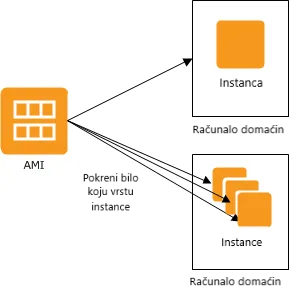
\includegraphics[scale=0.6]{imgs/ami}
	\caption{AMI predložak i distribucija slika stroja na instance \cite{ec2}}
	\label{fig:ami}
\end{figure}

AMI predlošci podržavaju dva tipa virtualizacije: hardversku virtualizaciju i paravirtualizaciju. Predložak s hardverskom virtualizacijom pruža mogućnost pokretanja operacijskog sustava izravno na vrhu virtualnog stroja bez ikakvih izmjena, kao da se pokreće na samom hardveru \engl{bare-metal hardware}. Domaćinski sustav usluge EC2 emulira dio ili sav temeljni hardver koji je predstavljen gostu odnosno AMI slici. Moguće je isto tako koristiti hardverska proširenja koji pružaju brzi pristup domaćinskom hardveru. Paravirtualizacija koristi poseban pokretački program koji lančano učitava jezgru u AMI sliku. Paravirtualni gosti mogu se pokretati na domaćinskom hardveru koji nema eksplicitnu podršku za virtualizaciju. Ovaj tip ne simulira hardver, nego pravi hiperpozive \engl{hypercalls} za izvršavanje osjetljivih CPU naredbi. Preporuča se odabir hardverske virtualizacije, iako generalno paravirtualizacija pruža bolje performanse, zbog poboljšanja hardverske virtualizacije i novih upravljačkih programa koji izjednačava rad obje vrste virtualizacije. 

Pri kreiranju instance potrebno je definirati i njezinu vrstu. Vrsta koja se navede određuje hardver dostupan instanci. Svaka vrsta nudi različitu ravnotežu računalnih, memorijskih i mrežnih resursa. Vrste su grupirane u skupine na temelju potreba ciljnih aplikacija. AWS pruža sljedeće vrste instanci:
\begin{itemize}
	\item opće namjene \engl{general purpose}, 
	\item optimiziranog računanja \engl{compute optimized},
	\item optimizirane memorije \engl{memeory optimized},
	\item optimizirane pohrane \engl{storage optimized}, 
	\item ubrzanog računanja \engl{accelerated computing},
	\item računanja visokih performansi \engl{high-performance computing}.
\end{itemize}

Vrstu instance potrebno je odabrati na temelju zahtjeva same aplikacije. Isto tako, pri kreiranju instance, uvijek je potrebno voditi računa o odabiru regije - optimalno je odabrati regiju kojoj je klijentski promet najbliži.

Za potrebe razvijenog sustava, kreirana je EC2 instanca opće namjene s najmanjim resursima budući da je klijentski promet jako malen, odnosno vrlo malo korisnika pristupa aplikaciji. Također, pridružena joj je instanca spremnika za pohranu veličine 8 GB. Operacijski sustav na kreiranoj instanci aplikacije jest Linux radi lakšeg spajanja na instancu i pokretanja web aplikacije putem komandne linije. Pri stvaranju instance kreirana je nova sigurnosna grupa koja omogućava spajanje na virtualno računalo putem SSH klijenta.

Instanci je automatski dodijeljena virtualna privatna mreža \engl{Virtual Private Cloud - VPC} koja predstavlja izolirani virtualni mrežni prostor unutar AWS infrastrukture. Omogućava potpunu kontrolu nad mrežnim okruženjem, uključujući izbor vlastitog IP adresnog prostora, konfiguraciju podmreža, postavljanje usmjeravanja i pristupnih kontrola mreže. Svaka je virtualna privatna mreža podijeljena na manje dijelove mreže zvane podmreže. One mogu biti privatne ili javne te se automatski za svaku mrežu kreiraju tri podmreže. Svaka je kreirana podmreža prema zadanim postavkama privatna, te je za pristup instanci odnosno aplikaciji koja se nalazi za njom potreban javni pristup. Iako omogućavanje javnog pristupa znači da svatko može pristupiti IP adresi instance s interneta, unošenje IP adrese pri svakom pristupu aplikaciji nije prilagođeno korisniku, što narušava korisničko iskustvo korištenja aplikacije. Stoga je potrebno uvesti komponentu za balansiranje opterećenja \engl{load balancer}. Balanseri preusmjeravaju korisničke zahtjeve na manje opterećene instance i tako ravnomjerno raspoređuju ulazni promet. Budući da je u razvijenom sustavu korištena samo jedna instanca na kojoj se pokreće aplikacija, ovdje je primarna svrha balansera pružiti DNS naziv koji će biti javno dostupan korisnicima, i tako poboljšati iskustvo korištenja aplikacije. 

Aplikacijskoj instanci potrebno je dodijeliti pravila za ulazne zahtjeve, odnosno omogućiti TCP komunikaciju s podmreže u kojoj se nalazi balanser. Tim se pravilom omogućuje prolaz zahtjeva s balansera prema aplikacijskoj instanci. Isto tako, iz sigurnosnih razloga poželjno je koristiti protokol HTTPS za pristup balanseru. Za korištenje protokola HTTPS potrebno je učitati certifikat, no budući da domena na kojoj se nalazi balanser nije službeno registrirana, ne posjeduje niti službeno potpisani certifikat. Stoga je lokalno kreiran samopotpisani certifikat pomoću biblioteke \textit{OpenSSL} i zatim učitan u oblak. Slika \ref{fig:load_balancer} prikazuje mrežnu povezanost balansera i instance na kojoj se nalazi aplikacija. Balanser sluša promet na vratima 443, što su vrata za protokol HTTPS. Dolazni zahtjevi prosljeđuju se skupini ciljnih instanci, ovdje pod nazivom \textit{GrafanaTargetGroup}, u kojoj se mogu nalaziti sve buduće stvorene instance na kojima se pokreće aplikacija. Nadalje, promet se prosljeđuje ciljnoj instanci koja je dostupna na vratima 3000. Na tim je istim vratima pokrenuta aplikacija. 

\begin{figure}[ht]
	\centering
	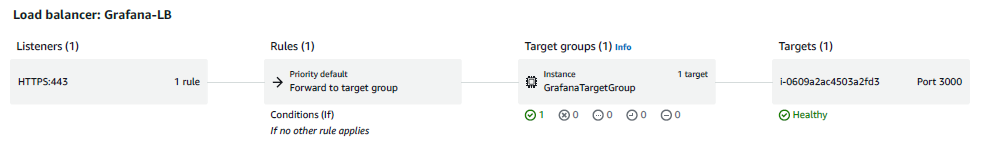
\includegraphics[scale=0.7]{imgs/load_balancer}
	\caption{Mrežna povezanost balansera i aplikacijske instance}
	\label{fig:load_balancer}
\end{figure}

Kako bi se maksimalno izoliralo izvođenje aplikacije i tako ostavilo prostora za izvršavanje drugih procesa na virtualnom računalu, na instanci EC2 aplikacija je pokrenuta pomoću alata Docker radi kontejnerizacije aplikacije. Sljedeći programski isječak prikazuje naredbu za preuzimanje i pokretanje Docker slike za Grafanu. Isto tako, potrebno je izložiti vrata na kojoj se pokreće aplikacija kako bi joj se moglo pristupiti. Grafana nudi dvije verzije - otvorenog koda i \textit{enterprise}, koja nudi više značajki. Za potrebe razvijenog sustava korištena je slika verzije otvorenog koda.

\begin{lstlisting}[caption={Pokretanje Docker slike za Grafanu}, language=bash]
	docker run -d -p 3000:3000 --name=grafana grafana/grafana-oss
\end{lstlisting}

\section{Grafana}

Grafana je platforma otvorenog koda za vizualizaciju i analizu podataka koja omogućava korisnicima stvaranje interaktivnih i prilagodljivih nadzornih ploča \engl{dashboards}. Cilj platforme jest olakšati analize vremenskih nizova podataka te integrira podatke iz različitih izvora podataka \engl{data source}, što mogu biti različite baze ili sustavi. Nudi jednostavnu vizualizaciju pomoću različitih grafičkih elemenata, uključujući linijske, stupčaste i tortne grafove. Široko je korištena zbog svoje sposobnosti da prezentira podatke na intuitivan način, omogućujući korisnicima donošenje informiranih odluka na temelju stvarnim podataka u stvarnom vremenu. Također, Grafana nudi alarmni sustav koji se koristi za izvještavanje korisnika o promjenama u podacima \cite{grafana}. 

Grafana se najčešće koristi za nadzor infrastrukture, performansi aplikacija i poslovnih metrika. Često je korištena za praćenje stanja poslužitelja, mrežnog prometa i performansi aplikacija. Također se koristi u poslovnoj analitici za praćenje poslovnih metrika. Isto tako, Grafana je korisna za IoT sustave upravo zbog sposobnosti vizualizacije velike količine podataka u stvarnom vremenu. Količine podataka koje IoT uređaji generiraju moraju se analizirati kako bi se dobili uvidi u očitana mjerenja, zdravlje sustava, kao i same performanse uređaja. Upravo zbog jednostavnog povezivanja s više različitih izvora podataka, njome se ostvaruje središnje mjesto za praćenje i analizu podataka iz cijele IoT mreže. Koristeći interaktivne nadzorne ploče, moguće je pratiti očitanja sa senzora u stvarnom vremenu i kreirati mnoge vizualizacije ovisno o potrebama sustava. Također podržava složene upite i transformacije podataka, što omogućuje njihovu dubinsku analizu. Korištenjem grafičkih elemenata i filtriranja podataka, mogu se lako identificirati trendovi, obrasci i anomalije u podacima \cite{grafana_iot}.

Kako bi web aplikacija mogla prikazivati podatke iz baze InfluxDB, na Grafani je potrebno stvoriti izvor podataka koji će služiti kao spojnica aplikacije i baze. Budući da se u bazi nalaze dvije kante, \textit{esp32data} i \textit{esp32state}, za svaku je od njih potrebno napraviti poseban izvor podataka. Kako bi se Grafana uspješno spojila na bazu, potrebno je korisničko ime i lozinka, kao i token koji će omogućavati čitanje iz baze. U bazi InfluxDB kreiran je novi korisnik \textit{grafana} koji služi samo za potrebe web aplikacije i generirana su dva tokena, svaki za jednu kantu. Tokeni omogućavaju isključivo čitanje iz kante. Važno je također napomenuti kako se novi korisnici ne mogu kreirati putem sučelja baze InfluxDB, nego je potrebno lokalno preuzeti alat za upravljanje bazom te se udaljeno putem komandne linije spojiti na bazu InfluxDB i tako kreirati korisnika.

Za kreiranje upita prema bazi koristi se jezik Flux. To je skriptni jezik za podatke \engl{functional data scripting language} namijenjen postavljanju upita i analizi podataka vremenskih serija. Upiti mogu sadržavati agregacije i transformacije. Iako jezik dolazi sa predefiniranim skupom funkcija za rad nad vremenskim serijama, moguće je definirati i vlastite prilagođene funkcije. Većina upita u jeziku Flux prate jednaki slijed koji se lančano izvodi:
\begin{enumerate}
	\item definiranje izvora,
	\item filtriranje,
	\item oblikovanje,
	\item obrada. 
\end{enumerate}

Prvi korak je odabir izvora podataka, što se odnosi na izbor kante. Podaci su vraćeni u tabličnom obliku. Funkcije filtriranja iteriraju po svim redovima dobivene tablice i provjeravaju zadovoljavaju li unosi tražene kriterije. Primarne funkcije za filtriranje su \lstinline|range()| i \lstinline|filter()|. Prva funkcija filtrira podatke na temelju vremenskog okvira, dok \lstinline|filter()| filtrira vrijednosti na temelju sadržaja redaka. Koristi se predikatna funkcija definirana unutar izraza za evaluaciju retka. Svaki se redak predikatnoj funkciji prosljeđuje kao zapis koji sadrži parove ključ-vrijednost za svaki stupac u retku. Oblikovanje podataka odnosi se na grupiranje ili modifikaciju same strukture podataka prije slanja na daljnju obradu. Funkcija \lstinline|group()| grupira podatke na temelju danog ključa, \lstinline|window()| stvara skupine na temelju danih vremenskih okvira, dok \lstinline|keep()| i \lstinline|drop()| zadržavaju odnosno uklanjaju pojedine stupce. Funkcija \lstinline|pivot()| vrijednosti stupca pretvara u redak. Obrada podataka odnosi se nad sve ostale operacije manipulacije podacima: agregiranje, mapiranje, prepisivanje te odabir pojedinih točaka u vremenu \cite{influxdb}. 

\subsection{Alarmni sustav}

%Gotovo sigurno ću koristiti Grafanu budući da ima gotove vizualizacije koje su meni potrebne. Isto tako, malo opisati funkcionalnosti koje se nude u samoj Grafani, kako funkcionira alerting sustav. Napraviti nekoliko dashboarda, povezati s datasourceom, kreirati par alerta i pokazati kak su došli u obliku maila. Ponuditi proširenja za to - PagerDuty aplikacija recimo. Opsgenie. Pogledati On Call plugin za Grafanu, jel potreban i jel koristan. 